\chapter{System Architecture}
This chapter introduces the architecture of \acrlong{ew} and provides a high-level overview of its components, each designed to satisfy the requirements outlined in \cref{chap:requirements}. \acrshort{ew} employs a hybrid architecture that combines on-chain and off-chain elements, thereby delivering a user-friendly, secure and technologically advanced academic record system. The integrated components, illustrated in \cref{fig:baseArchDiag}, are:
\begin{itemize}
    \item \textbf{Smart Contracts}: A suite of on-chain contracts that implement the core system logic, including the creation of students and university accounts creation and the management and retrieval of academic records. 
    \item \textbf{Browser Extension}: A graphical interface through which students can manage their academic wallets and interact with their records.
    \item \textbf{\acrfull{sdk}}: A TypeScript library intended for integration into university \acrshort{lms}, facilitating seamless interaction with \acrshort{ew}'s blockchain components.
    \item \textbf{Decentralized Storage System}: An off-chain solution for storing and retrieving certification files, which reduces on-chain storage costs by handling large documents externally.
\end{itemize}
\begin{figure}[htpb]
  \centering
  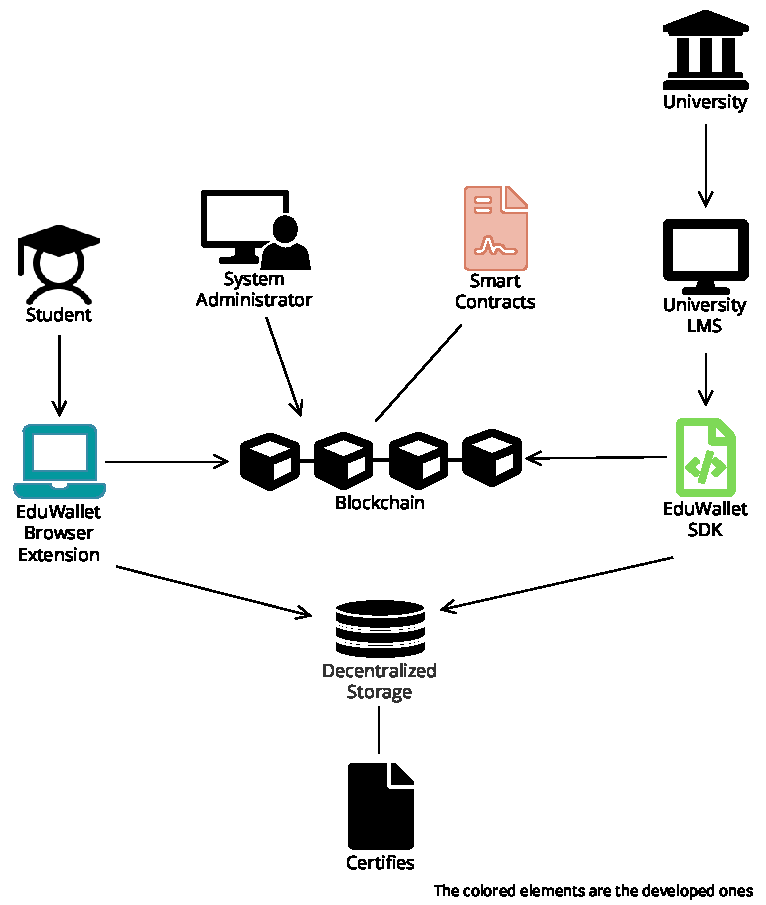
\includegraphics[width=0.6\textwidth]{figures/Architecture diagram basic.pdf}
  \caption[System basic architecture diagram]{Base architecture of the \acrlong{ew} system}
  \label{fig:baseArchDiag}
\end{figure}
In addition to these core components, we developed a simple yet complete \textbf{\acrfull{cli}}, which serves as a testing and demonstration tool and enables users to perform all operations typically available to universities, thereby simplifying the interaction with our \acrshort{sdk}. Because the focus of our work is on the interaction of universities and students with the academic registry, the system administrator's core functionalities\footnote{The approval and subscription of universities} have been inserted directly in the \acrshort{cli}. This design decision streamlines our use case and reduces unnecessary complexity.

The next chapters provide a detailed breakdown of the on-chain (\cref{chap:onchainDesign}) and off-chain (\cref{chap:offchainDesign}) designs.